\documentclass[10pt]{standalone}
\usepackage{amsmath}
\usepackage{amssymb}
\usepackage[utf8]{inputenc}
\usepackage{pgf,tikz,pgfplots}
\pgfplotsset{compat=1.15}
\usetikzlibrary{arrows}
\pagestyle{empty}
\begin{document}

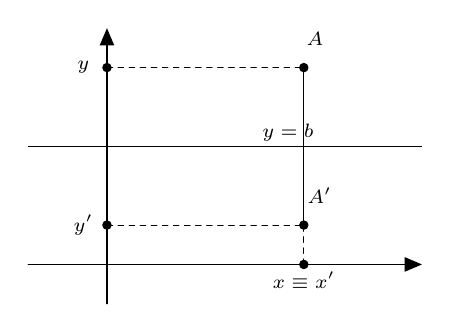
\begin{tikzpicture}[line cap=round,line join=round,>=triangle 45,x=1.0cm,y=1.0cm]
\draw[->] (-1.,0.) -- (4.,0.);
;
\draw[->] (0.,-0.5) -- (0.,3.);
\clip(-1.,-0.5) rectangle (4.,3.);
\draw [domain=-1.:4.] plot(\x,{(--1.5-0.*\x)/1.});
\draw [dash pattern=on 2pt off 2pt] (0.,2.5)-- (2.5,2.5);
\draw [dash pattern=on 2pt off 2pt] (0.,0.5)-- (2.5,0.5);
\draw [dash pattern=on 2pt off 2pt] (2.5,0.0)-- (2.5,0.5);
\draw (2.5,2.5)-- (2.5,0.5);
\begin{scriptsize}

\draw [fill=black] (2.5,2.5) circle (1.5pt);
\draw[color=black] (2.64,2.87) node {$A$};
\draw [fill=black] (2.5,0.5) circle (1.5pt);
\draw [fill=black] (2.5,0.0) circle (1.5pt);
\draw[color=black] (2.5,-0.2) node {$x\equiv x'$};
\draw[color=black] (2.7,0.87) node {$A'$};
\draw [fill=black] (0.,2.5) circle (1.5pt);
\draw[color=black] (-0.3,2.5) node {$y$};
\draw [fill=black] (0.,0.5) circle (1.5pt);
\draw[color=black] (-0.3,0.5) node {$y'$};

\draw[color=black] (2.3,1.67) node {$y=b$};
\end{scriptsize}

\end{tikzpicture}
\end{document}